%%%%%%%%%%%%%%%%%%%%%%% file template.tex %%%%%%%%%%%%%%%%%%%%%%%%%
%
% This is a general template file for the LaTeX package SVJour3
% for Springer journals.          Springer Heidelberg 2010/09/16
%
% Copy it to a new file with a new name and use it as the basis
% for your article. Delete % signs as needed.
%
% This template includes a few options for different layouts and
% content for various journals. Please consult a previous issue of
% your journal as needed.
%
%%%%%%%%%%%%%%%%%%%%%%%%%%%%%%%%%%%%%%%%%%%%%%%%%%%%%%%%%%%%%%%%%%%
%
% First comes an example EPS file -- just ignore it and
% proceed on the \documentclass line
% your LaTeX will extract the file if required
%\begin{filecontents*}{example.eps}
%!PS-Adobe-3.0 EPSF-3.0
%%BoundingBox: 19 19 221 221
%%CreationDate: Mon Sep 29 1997
%%Creator: programmed by hand (JK)
%%EndComments
%gsave
%newpath
%  20 20 moveto
%  20 220 lineto
%  220 220 lineto
%  220 20 lineto
%closepath
%2 setlinewidth
%gsave
%  .4 setgray fill
%grestore
%stroke
%grestore
%\end{filecontents*}
%
\RequirePackage{fix-cm}
%
%\documentclass{svjour3}                     % onecolumn (standard format)
%\documentclass[smallcondensed]{svjour3}     % onecolumn (ditto)
\documentclass[smallextended]{svjour3}       % onecolumn (second format)
%\documentclass[twocolumn]{svjour3}          % twocolumn
%
\smartqed  % flush right qed marks, e.g. at end of proof
%
\usepackage{graphicx}
\usepackage{tabulary}
%
%\usepackage{mathptmx}      % use Times fonts if available on your TeX system
%
% insert here the call for the packages your document requires
%\usepackage{latexsym}
%\usepackage{amsmath}
%\usepackage{amsthm}
\usepackage{color}
\usepackage{caption}
\usepackage{float}
%\usepackage{subfigure}
\usepackage{amssymb}
\usepackage{multirow}
\usepackage{multirow}
%\usepackage{subcaption}
%MRS2: check the appropriate natbib options to give the type of citations JCAMD has (bracketed numbers)
\usepackage[numbers, square,sort&compress]{natbib}
\graphicspath{{figures/}}
%
% please place your own definitions here and don't use \def but
\newcommand{\BibTex}{\textsc{Bib}\TeX}
\newcommand{\erfc}{\mathrm{erfc}}
%
% Insert the name of "your journal" with
\journalname{JCAMD}
%
\begin{document}

\title{Considerations when comparing molecular dynamics simulation engines: lessons learned in the automated conversion of input files for SAMPL5}
%\thanks{Grants or other notes
%about the article that should go on the front page should be
%placed here. General acknowledgments should be placed at the end of the article.}
%\subtitle{Do you have a subtitle?\\ If so, write it here}

\titlerunning{Considerations when comparing molecular dynamics simulation engines}        % if too long for running head

\author{Michael R. Shirts \and Christoph Klein \and Jason M. Swails \and Jian Yin \and Michael K. Gilson \and David L. Mobley \and David A. Case \and Ellen D. Zhong}

\authorrunning{M. R. Shirts et al.} % if too long for running head

\institute{Michael R. Shirts \at
              Department of Chemical and Biological Engineering, University of Colorado Boulder,
              Boulder, Colorado, USA 
		\email{michael.shirts@colorado.edu}
           \and Christoph Klein \at
              Department of Chemical Engineering, Vanderbilt University, Nashville, TN, USA
              \and Jason M. Swails \at Department of Chemistry and Chemical Biology, Rutgers University, Rutgers, NJ, USA  % no currently there, but most of the work was performed here?  Jason, let me know what your thoughts are on this   
              \and Jian Yin \at Skaggs School of Pharmacy and Pharmaceutical Sciences, University of California, San Diego, CA, USA
              \and Michael K. Gilson \at Skaggs School of Pharmacy and Pharmaceutical Sciences, University of California, San Diego, CA, USA
              \and David L. Mobley \at Departments of Pharmaceutical Sciences and Chemistry, University of California, Irvine, Irvine, CA, USA
              \and David A. Case \at Department of Chemistry and Chemical Biology, Rutgers University, Rutgers, NJ, USA
              \and Ellen D. Zhong \at Department of Chemical Engineering, University of Virginia, Charlottesville, VA, USA % essentially all the work was done when in my group, and Shaw may have issues with their name appearing somewhere else. 
}

\date{Received: date / Accepted: date}
% The correct dates will be entered by the editor


\maketitle

% use \label to label figures, and \ref to refer to these labels.  Don't directly use figure numbers!  also better to use figure names (fig:bestfit vs fig:2) to keep from confusing things.
%
\begin{abstract}

We describe the efforts to prepare common starting structures and
models for the SAMPL5 blind prediction challenge. We generated the
starting input files and single configuration potential energies for
the host-guest and distribution coefficient molecules in the SAMPL5
blind prediction challenge for the GROMACS, AMBER, LAMMPS, DESMOND and
CHARMM molecular simulation programs. All conversions were fully
automated from the originally prepared AMBER input files using a
combination of the ParmEd and InterMol conversion programs.

We find that all programs agree to a large extent when reasonable
choices are made for different cutoff parameters, though some
surprising sources of statistically significant differences occur. For
example, differing choices of Coulomb's constant in each program is
one of the largest sources of discrepancies in energies between the
programs. We discuss the measures required to get good agreement in
the energies for equivalent starting configurations between the
simulation programs, and the energy differences that occur when
simulations are run at their program-specific default values. Finally,
we discuss was was required to automate this conversion and
comparison.

\keywords{molecular dynamics, simulation validation, molecular simulation}
% \PACS{PACS code1 \and PACS code2 \and more}
% \subclass{MSC code1 \and MSC code2 \and more}
\end{abstract}

\newpage
\section*{Introduction}
\label{intro}

The goal of the ongoing SAMPL blind prediction
challenges~\citep{Muddana2014SAMPL4,Muddana2012a,geballe_sampl2_2010,guthrie_blind_2009}
is to compare purely computational blind predictions of thermodynamic
properties, such as hydration free energies, partition coefficients,
and binding free energies, for a range of both model and more realistic
situations. Such blind prediction challenges can be very useful in
identifying unexpected reasons for differences between methods that
should, in theory, yield the same result. For example, even when the
same program is used with what is listed as the same force field,
significant differences can be obtain. In the SAMPL4 blind test, two
different sets of simulations performed with GROMACS, TIP3P water, and
GAFF/AM1-BCC parameterization had differences of $0.5 \pm 0.1$
kcal/mol that were ultimately tracked down to whether the large host
molecule had AM1/BCC partial charges determined fragment-wise or for
the entire molecule at the same time, the level of detail that often
does not make it into publication.~\cite{Monroe2014}

One particular question that can be difficult to address is to what
extent methods that are supposed to be identical will give different
results with different simulation programs.  Therefore, one of the
tasks carried out in preparation for SAMPL5 was to prepare starting
simulations in several of the most common molecular simulation
packages (AMBER~\citep{???}, GROMACS~\citep{hess_gromacs_2008},
LAMMPS~\citep{plimpton_fast_1995},
DESMOND~\citep{bowers_scalable_2006}. To ensure that the simulations
were translated correctly, it was also necessary to compare the
evaluated energies of the initial configurations in the native
simulation programs for each file format to ensure that the
translation had been done correctly.  This also involved an analysis
of which different simulation conditions and parameter choices were
necessary for these simulation programs to give the same, or
substantially the same, energy.  In order to make this task feasible,
this process was necessarily highly automated. We present here the
results of this comparison. One important change from the initial work
carried out for SAMPL5 and this one is adding the generation of
CHARMM-format starting files as well as the initial energies generated
with the CHARMM simulation program.

In this study, we have chosen to compare only the energies of initial
structures and not the values of thermodynamic observables such as
average energy, nor more complicated physical observables such as
hydration free energies which require multiple simulations.  The
reason for limiting this study to the evaluation of single point
energies is to better deconvolute the different tasks that molecular
simulation engines perform.

The first task that a molecular simulation engine has is to take an
molecular configuration and a model (i. e. a specification of all
force field parameters) and from these ingredients generate the energy
of the model in that configuration and, in molecular dynamics
approaches, also the forces acting on each particle.  Next, given the
assignment of energies and forces to a configuration, a molecular
simulation engine then also generates a sequence of configurations
that belong to a desired ensemble of that model, such as the
microcanonical (NVE), canonical (NVT), or isobaric-isothermal (NPT)
ensemble, with their corresponding probability distribution for each
configuration.

However, this second task requires a large number of different
decisions that are made mostly independently of the assignment of
energy to a set of coordinates.  Slightly different integration
methods will give rise to slightly different
ensembles.~\citep{???} To pick one example, molecular dynamics
averages are slightly dependent on the time step, and using longer
time steps means the simulation is occurring at a slightly higher
effective temperature, which may or may not be detected in the
temperature estimator of the simulation.~\citep{???} Different
thermostats will converge to the correct ensemble (if they are
actually correctly implemented thermostats) but the speed at which
they approach to that value can vary. Different programs have
different recommended integration schemes. Addressing the multitude of
possible ways that simulations could differ using different
integration schemes is beyond the scope of this study.


Additionally, a difference between the output of programs with
theoretically the same model occurs when the energy and forces are
approximated in order to increase the number of molecular dynamics or
Monte Carlo steps in a fixed amount of computing time. For example,
Lennard-Jones terms may be truncated at some separation distance
distance with some sort of approximation for longer
distances~\citep{AllenAndTildesley,shirts_accurate_2007,wu_isotropic_2005},
or Coulombic interactions long-range terms may be approximated by an
interpolated mesh~\citep{essmann_smooth_1995} rather than a direct
lattice sum.  Not only does each program make different default
choices, most of these choices are left up to the user, meaning
different results can be obtained by different users of the same code,
and the recommended or default behavior of each code will almost
certainly differ from program to program to some degree.

Understanding what the effect of the choice of such a wide range of
approximations for even simple quantities such as enthalpy or density
is extremely time-consuming, and has only been done partially
systematically. Simulation observables are ensemble averages, and are
thus statistical quantities with associated statistical error. Since
the uncertainty scales as (simulation time)$^{-1/2}$, increasing the
accuracy by a factor of 10 requires 100 times as much simulation
time. Small differences in the parameters used to run the simulations
simulations give rise to similarly small changes in the ensemble
averages. If we attempt to calculate a small difference between
ensemble averages $\langle O \rangle_1$ and $\langle O \rangle_2$,
carried out at simulation parameter sets 1 and 2, with statistical
uncertainties $\sigma_1$ and $\sigma_2$, the error in $\langle O
\rangle_1 - \langle O \rangle_2$ will be
$\sqrt{\sigma_1^2+\sigma_2^2}$. If $\langle O \rangle$ is, for
example, the enthalpy of a calculation, it might be of order -100,000
kJ/mol.  For a given amount of simulation time, if the relative error
in $\langle O \rangle$ is 0.0001\% or about 10 kJ/mol, then error in
$\langle O\rangle_1 - \langle O \rangle_2$ will be of order 14
kJ/mol. Clearly, it would be important to know if a change in a
simulation parameter changed the an enthalpy difference by anywhere
near 14 kJ/mol. To take that uncertainty down to, say, a 95\%
confidence interval of 1 kJ/mol would take approximately $(2\times
14)^2 \approx 800$ times as much simulation as determining $\langle O
\rangle$ itself to one part in 10$^{-6}$.  Reweighting approaches have
recently been developed to include the correlation between variables,
allowing in may cases the uncertainty to be calculated by one to three
orders of magnitude more efficiently.~\cite{Paliwal2013} However, even
with this acceleration, it is still extremely expensive. For this
additional reasons, enumerating all the possible ways that simulation
parameters affect ensemble observables is beyond the scope of this
study.

Such comparisons are even harder for simulations requiring multiple
simulations, such as free energy calculations to obtain solvation free
energies or binding affinities~\cite{???}.  The expense of such
approaches requires the development of significant new methodologies
in order to obtain reasonably efficient results for parameter
sensitivity tests of free energies~\cite{naden_rapid_2016}. These more
complex observables are calculated using a large number of different
methodologies, all of which have new parameters, with different
statistical accuracies and inherent biases. The number of different
approaches with different domains of applicability can significantly
confound the ability to truly understand the effect of underlying
assumptions.

This lack of systematic study of the effect of many of these
approximations is partly due to the fact that most choices actually do
not have significant effects on simulation observables. The main
reason for this is that many default choices were made with good
underlying physical reasoning, and thus lead to relatively comparable
and reliable results. This makes it rather unrewarding to carry out
such computationally intensive searches to find the few choices that
do significantly affect simulation observables.  

However, another reason for the lack of systematic study of molecular
simulations is the fact that unless the underlying energy functions
are the same between different programs, then it is very difficult to
compare the results obtained for sensitivity of a given setting
obtained with one program with that obtained by a separate program.
It is always challenging to obtain comparable results using one
simulation engine with a second simulation engine, because the input
configurations and model must be converted, which either is done using
painstaking manual copy-and-pasting, one-off scripts, or occasionally
existing scripts that can convert from one specific program to
another.  Some examples include ACPYPE, a converter from AMBER to
GROMACS~\citep{sousa_da_silva_acpype_2012},
CHAMBER~\citep{crowley_chamber:_2009} a converter from CHARMM to
AMBER, {\tt amber2lmp}, a script converting between LAMMPS and AMBER
files. [NOTE: what am I missing?] There are other resources which do not convert directly, but
will build the same system in multiple programs, such as
CHARMM-GUI.~\citep{lee_charmm-gui_2016}

In this study, we will therefore focus on the automated conversion of
molecular simulation input files using to the extent possible
automated all-to-all conversion tools, and the comparison and
validation of the energies of single configurations among these
programs.  This validation serves as a necessary building block for
later studies to more easily evaluate the differences between
simulation engines in calculating simulation observables, and the
comparison of more advanced simulation methods between different
simulation programs.

\section*{Methods}
\begin{sloppypar}
The molecular intercoversion software programs InterMol
(https://github.com/shirtsgroup/InterMol) and ParmEd
(http://parmed.github.io/ParmEd/) were used to perform comparisons
between five different simulation input parameter files and engines.
InterMol is designed as a generalizable all-to-all converter between
molecular simulation file formats; however, it currently only has full
support for GROMACS, LAMMPS, and DESMOND file formats.  ParmEd is
[Jason: fill in more here] a molecular topology editor that also
provides conversion functionality between GROMACS, AMBER, and CHARMM
force field formats.
\end{sloppypar}

We took advantage of this overlap in conversion functionality to
provide output files in five formats. The process is as follows: We
took files initially parameterized in AMBER format using AmberTools
and read them using ParmEd. We then used ParmEd to convert them into
GROMACS input file formats. We then convert from these GROMACS files
into LAMMPS and DESMOND input files using InterMol.  ParmEd was also
used for this study (though not the original SAMPL5 release) to
convert the AMBER simulation files into CHARMM simulation files
directly.

We use the InterMol convert.py tool to manage all of the conversions
(including interfacing with the ParmEd API). InterMol allows control
of simulation input parameters by either reading a user-defined (or
default) sample simulation parameter file (for DESMOND, AMBER, and
GROMACS) or inserting user-defined strings defining nonbonded terms
into the parameter and topology files (LAMMPS and CHARMM). Full
any-to-any conversion is not yet possible using the combination of
tools so far, since ParmEd cannot yet convert between some dihedral
formats, making it impossible to write many valid GROMACS files into
CHARMM or AMBER formats.

We use the 22 host-guest molecules distributed as part of the SAMPL5
blind challenge, with 10 ligands bound to the CBClip, 6 ligands with
the octa-acid OAH host, and 6 ligands with the octa-acid OAMe
host.~\cite{mainSAMPL5paper} An idealized model of the 3D structure
of host CBClip was provided by Prof. Lyle Isaacs. The starting 3D
structures of hosts OAH and OAMe were built manually with MOE and
partly energy minimized. The initial structures of free guest
molecules were found via the conformational search feature in MOE. For
CBClip, the experimental studies were done at pH 7.4, so the host’s
four sulfonic acid acids were treated as fully ionized, for a net host
charge of -4.  For the octa-acids, OAH and OAMe, the experimental
studies were done at pH 11.5, so all eight carboxylic acids were
treated as fully ionized, for a net charge of -8. The protonation
states of all guest molecules were also assigned based on their
expected pKas and the experimental pH values, as shown in the figures
above, and were assumed to remain the same on binding their respective
hosts.

Partial charges were generated with the restrained electrostatic
potential (RESP) fitting procedure, with electrostatic potentials at
the HF/6-31G* level, as implemented in Antechamber.  Bonded and van
der Waals parameters were assigned by GAFF~\citep{wang_development_2004} in Antechamber. For the
octa-acids, which have a well-defined hydrophobic cavity, the bound
conformations were set up with the guests' ionized groups at the
opening and their hydrophobic parts in the cavity. For the CBClip
host, the positions of the guests in the binding site were constructed
by manual docking in MOE.  Each bound complex was placed in a cubic
simulation box with edge length of about 4 nm, and containing 2100
TIP3P (non-modified) water molecules. Sodium ions were added to
neutralize all systems. Given the low concentration of the buffer used
in experiments, no extra ions were added to mimic the buffer. The
sodium ions were modeled with the TIP3P-specific sodium parameters
of~\citep{Joung2008}. Each system was then subjected to a short equilibration
phase (first NVT, then NPT) to heat the system and change the volume
so the pressure would be about 1 atm. [MRS: how short? What was done
  precisely?] The solutes were restrained during the entire process,
so only the environment was relaxed. Note that the AMBER .rst7 files
contain velocities consistent with a temperature of 298.15 K.

For this study, the most up-to-date releases of all molecular dynamics
simulation programs were used. In most cases, this resulted in very
little difference in the results between the current study and the
SAMPL5 study, but in some cases as noted, the results do change. Units
are given in SI units (kJ/mol and nm, for example), though different
programs use different default units. [QUESTION TO ALL: what do people
  think about units? I'd rather not be switching back and forth from
  kJ/kcal and nm/\AA. And if I pick one set of units, SI would be the
  'right' one]

The five programs were:
\begin{itemize} 
\item {\bf AMBER}: Energies were calculated originally for SAMPL5, with
  {\tt sander} as included AmberTools 14, but for the current study
  {\tt sander} from the most recent AmberTools 16 were used.
\item {\bf GROMACS}: Energies were calculated originally and here with
  GROMACS 5.0.4, compiled in double precision.
\item {\bf DESMOND}: Energies were calculated in the original
  SAMPL5 release with 3.6012 (distributed as part of the Schr\"odinger
  2013 package for academic use) but all tests are performed here with
  version X version 4.5 (distributed as part of the Schr\"odinger
  2016-1 package for academic use).  Rather than directly writing the
  DESMOND .dms files, the automated conversion routines were written to
  create MAESTRO .cms files.
\item {\bf LAMMPS}: Energies were calculated with the April 5,
  2014 build in the SAMPL5 release, and the Feb 16, 2016 release in
  the current study. Only the additional modules to run atomistic
  simulations were installed.
\item {\bf CHARMM}: Energies were only generated for this study, with
  developmental version 40b2 of the charmm-lite free package.
\end{itemize}

All programs were compiled in RHEL 7 with the gcc 4.8.5 compiler
suite.

It is difficult to choose simulation parameters that agree among all
simulation engines: for example, each program generally has different
types of default switching functions to taper nonbonded
interactions. For this comparison, we therefore chose for our
nonbonded methods that were sufficiently cutoff independent that
differences in the cutoff scheme between programs would minimally
affect the results.

For electrostatic interactions, we chose either particle mesh Ewald
(PME) implementations (CHARMM, AMBER, GROMACS, CHARMM) or
particle-particle particle-mesh (PPPM) methods (LAMMPS). We chose a
cutoff of 1.5 nm for both Coulomb and van der Waals interactions to
eliminate much of the issues with errors at short range cutoffs. We
chose a real space error cutoff of $1\times 10^{-8}$, which corresponds
to a $\kappa$ (or $\beta$) parameter of 0.020822755 nm.  For PPPM, we
chose a tolerance of $1\times10^{-8}$, which was necessary to reduce
the error below [MRS: look up the numbers on this.] For AMBER and
CHARMM, we used a PME mesh grid of 48 $\times$ 48 $\times$ 48 grid
points with 4th order interpolation. DESMOND allows significantly less
control over the PME parameters at the MAESTRO interface level, and we
used a PME relative tolerance of $1\times 10^{-10}$ [MRS: look up what
  that setting means again]

For Lennard-Jones interactions, we avoid the problems of trying to
match switching schemes between programs, which are usually quite
different, by using an abrupt cutoff to zero potential. This approach
is not recommended for running molecular dynamics simulations, as it
creates a mismatch between forces and energies, but which is
reasonable for comparing simulation energies. An analytic isotropic
long-range correction was used for LAMMPS, AMBER, DESMOND, and
GROMACS~\citep{AllenAndTildesley,shirts_accurate_2007}, with the isotropic
periodic sum approach~\citep{wu_isotropic_2005} used for CHARMM.  At this longer
range, the results become essentially independent of the precise
cutoff for both methods, though the isotropic periodic sum is less
cutoff dependent, as seen in Table~\ref{table:ljcutchange}. This
cutoff independence is expected for systems that are homogeneous at
long range, such as a host-guest system surrounded by water, but will
not be cutoff independent for a heterogeneous system such as a lipid
bilayer or a liquid/vapor interface~\cite{veld_application_2007}.

\begin{table}
\caption{\label{table:ljcutchange}Using an analytical correction, the
  van der Waals energy due to the Lennard-Jones interactions are
  essentially independent of cutoff, with a total change of 0.001\% in
  the total van der Waals energy for the analytic long range
  correction in GROMACS (and similar to other programs) and and
  0.00008\% with the isotropic periodic sum in CHARMM, over a change
  of 0.3 nm cutoffs.}
\begin{tabulary}{\textwidth}{|C|CC|}
\hline
Distance (nm) & GROMACS  
Potential Energy (kcal/mol) & CHARMM Potential Energy (kcal/mol)\\
\hline 
1.5 & 2921.4840 & 2921.54699\\
1.4 & 2921.4923 & 2921.54623\\
1.3 & 2921.5265 & 2921.54597\\
1.2 & 2921.5246 & 2921.54456\\
\hline
\end{tabulary}
\end{table}

We also ran the test with an attempt to be as close to default
parameters as possible. For AMBER, we use a 0.9 nm cutoff, with the
same Ewald parameters (48$\times$48$\times$48 Fourier points in the
grid), with the isotropic analytical dispersion correction included
for Lennard-Jones [MRS: is this an abrupt cutoff, or is it scaled
  somehow?] For GROMACS, a Fourier spacing of 0.1 nm is used For
LAMMPS, we use pair\_style lj/cut/coul/long 9.0 9.0.  We include a
dispersion correction, and use PPPM, with $10^{-8}$ [MRS: right choice?].

We also examined how dependent the energy differences are on the
individual configurations. For twelve of the systems (the six OAMe and
the six OAH octa-acid host-guest systems), we take 20 different
configurations. These configurations were generated with electrostatic
parameters and Lennard-Jones parameters as listed in the 'default'
parameter section. Temperature was maintained at 298.15 K with the
Langevin thermostat with a damping constant $\gamma$ of 1 ps$^{-1}$
with a timestep of 2 fs with constrained bonds [JANE: is this correct
  on the constraints, or were just H-bonds constrained?]. Simulations
were started from the SAMPL5 example files and run for 2 ns, and
configurations were taken every 100 ps.

Matching the precision of the coordinates in the files used in
conversion is important to matching the energies. While keeping the
precision of the input files the same, we truncated the precision of
the output files by a varying number of digits of precision in order
to examine how the energy components are affected. Note that lower
precision files will not have an affect on ensemble averages if such
files are only used as starting points for simulation. But it will
matter quite a bit if output configurations are used for reanalyzing
energy contributions.

Another source of differences in energy relates to the precision of
the binary.  We therefore also compare the the deviation from the
program average for the same version of GROMACS compiled in double
precision (the precision that is used in the reference calculations)
and in single precision.

%The default interactions lead to energy differences of 2-10 kcal/mol
%for these systems - need to adjust
%the nonbondeds to the choices described.  see:
%http://ambermd.org/namd/namd\_amber.html as an example, but we needed
%choices that worked for all molecules simultaneously Nothing needed
%for bond/angle/dihedral -

%12 A -> 2921.5246 (all kcal/mol).  For electrostatics, we choose PME
%with nx=ny=nz=48, 15 A cutoff, PME electrostatics (note -- chose
%spacing originally for SAMPL5 with 0.1 for GROMACS, need to verify it
%doesn’t matter). Rtol and beta are related by $r_{tol} = \erfc(\beta
%r_{coul,cutoff})$, so for rtol =10$^-5$ (default for GROMACS and
%AMBER), then for $r_{coul}$ = 0.9 nm, $\beta$ = 0.03470459 nm$^{-1}$, and
%when r$_{coul}$ = 1.5 nm, then $\beta$ = 0.020822755) Short description of
%software: InterMol pre-release interfacing with ParmEd.
% was lammps 10^7?
\begin{table}
{\tiny
\begin{tabulary}{\textwidth}{C|CCCCCCCCCC}
\hline
 & \multicolumn{2}{c}{AMBER} & \multicolumn{2}{c}{GROMACS} &\multicolumn{2}{c}{LAMMPS}& \multicolumn{2}{c}{DESMOND}&\multicolumn{2}{c}{CHARMM}\\
\hline
  & default settings & ideal settings  & default settings & ideal settings  & default settings & ideal settings  & default settings & ideal settings  & default settings & ideal settings  \\
van der Waals cutoff & 1.5 nm, abrupt & 0.9 nm, abrupt & 1.5 nm, abrupt & 0.9 nm, abrupt & 1.5 nm, abrupt & 0.9 nm, abrupt & 1.5 nm, abrupt & 0.9 nm, abrupt & 1.5 nm, abrupt & 0.9 nm, abrupt \\
Coulombic cutoff & 1.5 nm real space & 0.9 nm real space & 1.5 nm real space & 0.9 nm real space & 1.5 nm real space & 0.9 nm real space & 1.5 nm real space & 0.9 nm real space & 1.5 nm real space & 0.9 nm real space \\
Long-range electrostatics & Ewald, Fourier points 48$\times$48$\times$48, order 4, real space error 10${-5}$ & Ewald, Fourier points 48$\times$48$\times$48, real space error 10${-5}$ & Ewald, Fourier points 48$\times$48$\times$48 & Ewald, Fourier spacing 0.1 nm & PPPM, 10$^{-8}$ tolerance & PPPM, 10$^{-8}$ tolerance & Ewald, 10$^{-10}$ relative tolerance & Ewald, 10$^{-10}$ relative tolerance &Ewald,  Fourier points 48$\times$48$\times$48 & Ewald, Fourier points 48$\times$48$\times$48 \\
Long-range van der Waals & Isotropic correction & Isotropic correction & Isotropic correction & Isotropic correction & Isotropic correction & Isotropic correction & Isotropic correction & Isotropic correction & Isotropic periodic sum & Isotropic periodic sum \\ 
\end{tabulary}}
\caption{Key nonbonded term setting for both default and ideal energy validation tests[NOTE: I'm not sure this table is the best way to summarize things.  Formatting is not ideal, obviously.]}
\end{table}

\section*{Results}
We first compare ten different energy terms between the five different
simulation programs with the ideal nonbonded parameters.  Results are
shown in Table~\ref{fig:mainfig}. All results are averaged over the 22
host-guest molecules included in the SAMPL5 blind prediction
challenge. To avoid picking a favored reference program, we look at
the deviation of each term from the average of all five programs,
calling this the ``program average'' for the molecule.  ``Potential
energy'' is the total potential energy of the system, but is not the
total over all 9 other energy terms, since several of these terms are
sums of other terms: ``Bonded'' is the sum of ``Bonds'', ``Angles'',
``All dihedrals'' (including both improper and proper dihedrals),
``Electrostatic'' is the sum of ``Coulomb 14'', Coulomb short range
and Coulomb long range forces, ``van der Waals'' is the sum of
``LJ-14'' and van der Waals short and long range terms, and
``Nonbonded'' is the sum of ``Electrostatic'' and ``van der Waals''
terms.

We examine three statistics to describe the deviations between the
programs: the average differences from the program average over all
molecules, the average of the absolute value of the difference from
the program average, and the average of the relative absolute value of
the difference. Each statistic gives somewhat different information
about the trials. The average gives information about the manner in
which energy component deviates from the program average, while the
absolute value of the differences shows the magnitude of the
deviation, avoiding any cancellation due to different signs.  Because
many terms are much smaller than others, for example, the bonded
energy terms being two to three orders of magnitude smaller than the
electrostatic term, the relative absolute difference shows the
fractional error in each term.

We find that the bonded terms match very well between all
programs. Average differences from the program average are below 0.05
kJ/mol in magnitude for all terms for all programs, and usually about
an order of magnitude lower, and around or below 0.002 kJ/mol (CHARMM
was slightly higher than the others), Average absolute differences in
the total bonded term are below 0.004 kJ/mol for all programs except
CHARMM. CHARMM's average absolute value is 0.007 kJ/mol, but is
dominated by differences in the dihedral terms; bond and angle terms
are as low as other programs.  Note that this is not per interaction,
but the sum over all interactions.

The average relative absolute quantities are perhaps a more important
comparison metric, since they are intensive quantities.  Total
deviation of the energy will of course become larger as the system
becomes larger, so normalizing by the total energy, which will be
proportional to system size, will result in a more useful comparison.
With this statistic, we see that the bonded terms are accurate to
generally about 3 parts in 10$^{-6}$, with CHARMM slightly higher at 7
parts in 10$^{-6}$. Given that this is approximately the limit of
precision one would see in single precision calculations, and given
the fact that some programs only output energies to four (AMBER) or
five (CHARMM) decimal places, or eight significant digits total
(LAMMPS) this seems for all programs to be a reasonable amount of
agreement in bonded interactions for most purposes. It demonstrates
that the conversion process has successfully copied parameters with
the correct functional form for bonded interactions between all of the
programs of interest, and the energies are being calculated in a
consistent way for these bonded interactions.  More generally, it
suggests that with no extra fiddling, all programs should in typical
cases generate essentially equivalent bonded energies.

\begin{figure}[h]
\begin{tabular}{c}
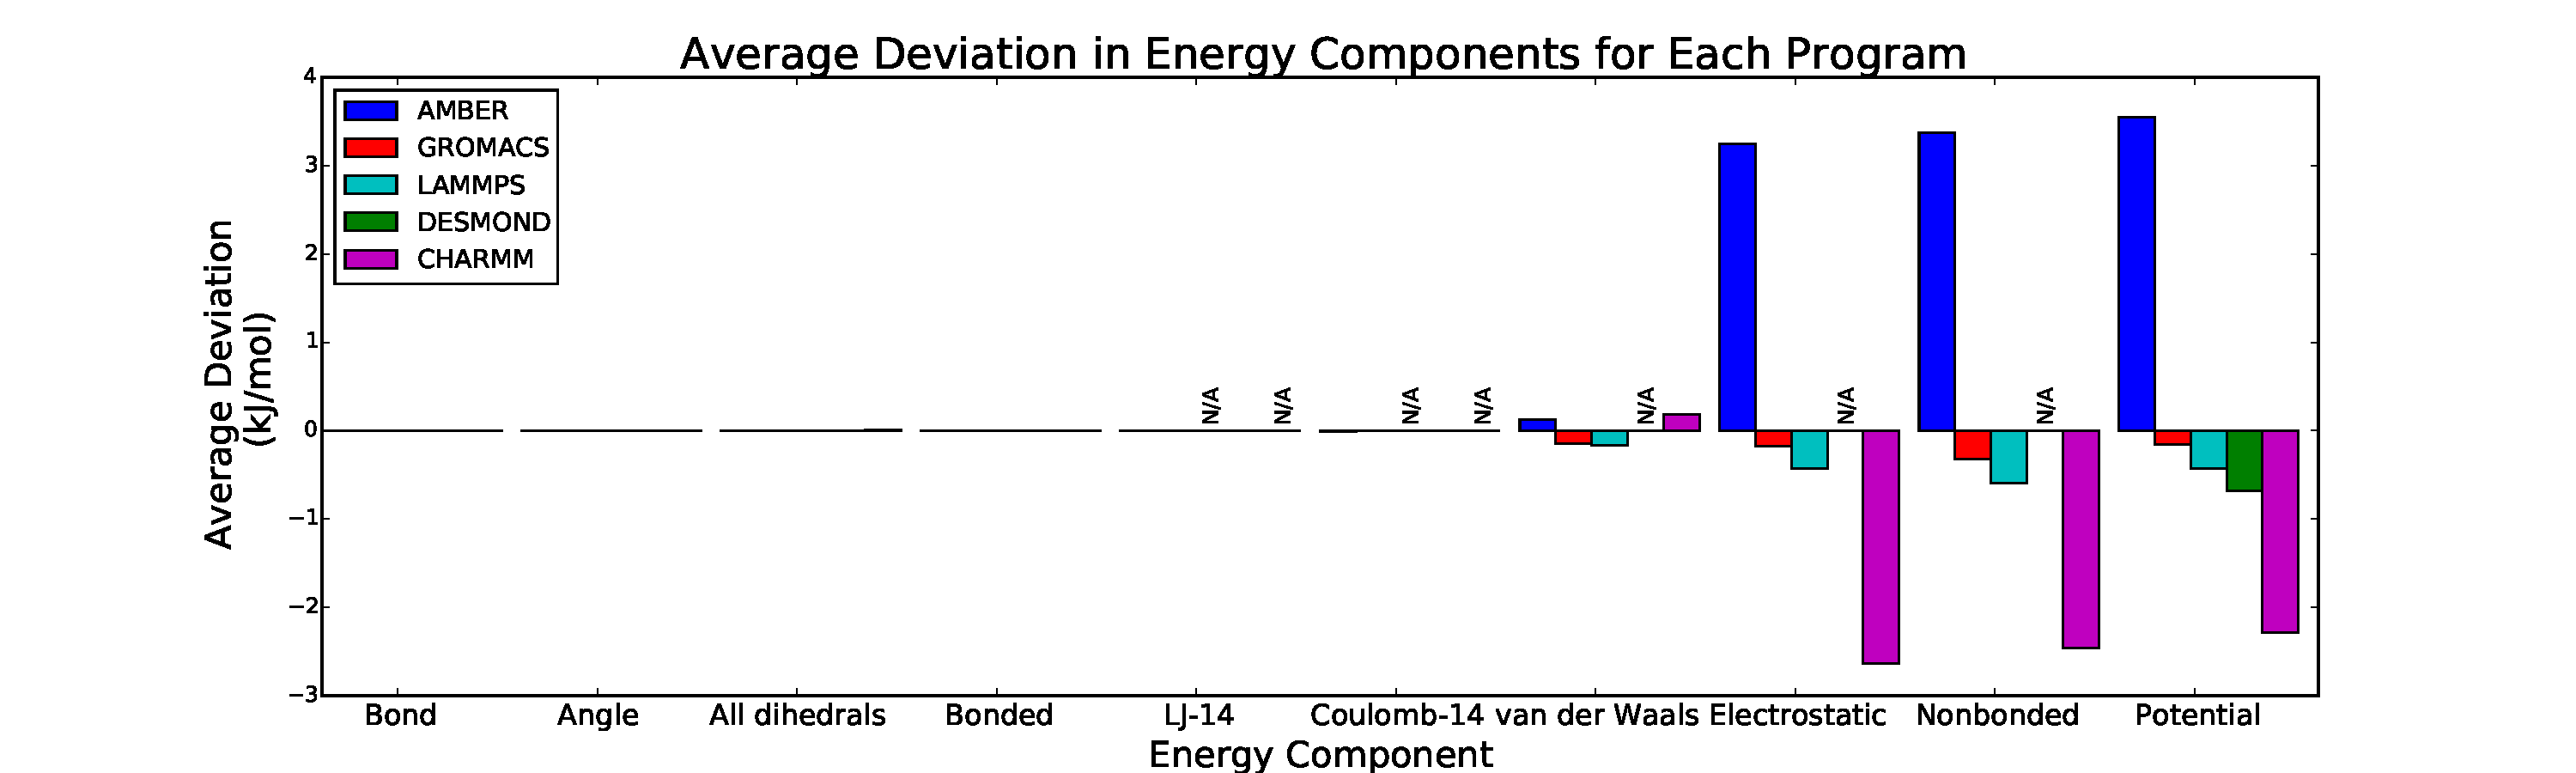
\includegraphics[width=\textwidth]{AverageIdealSettings.pdf} \\  
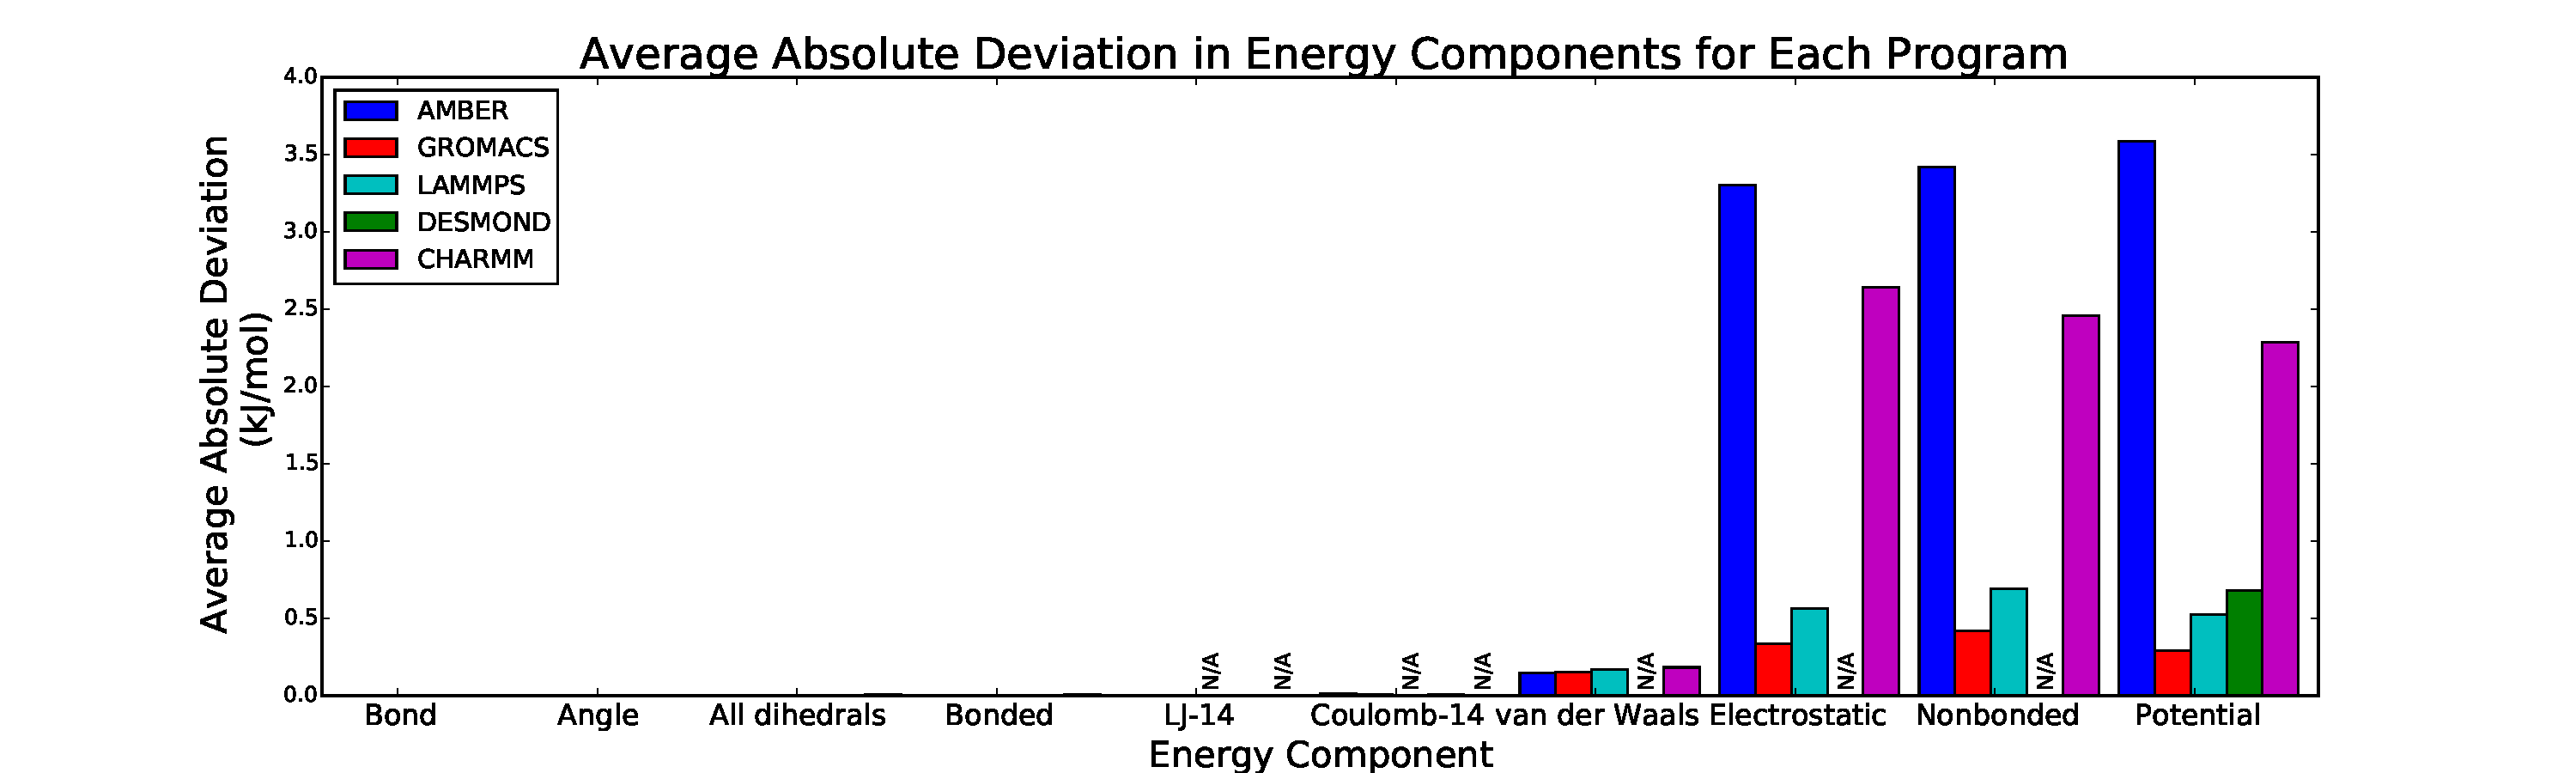
\includegraphics[width=\textwidth]{AverageAbsoluteIdealSettings.pdf} \\  
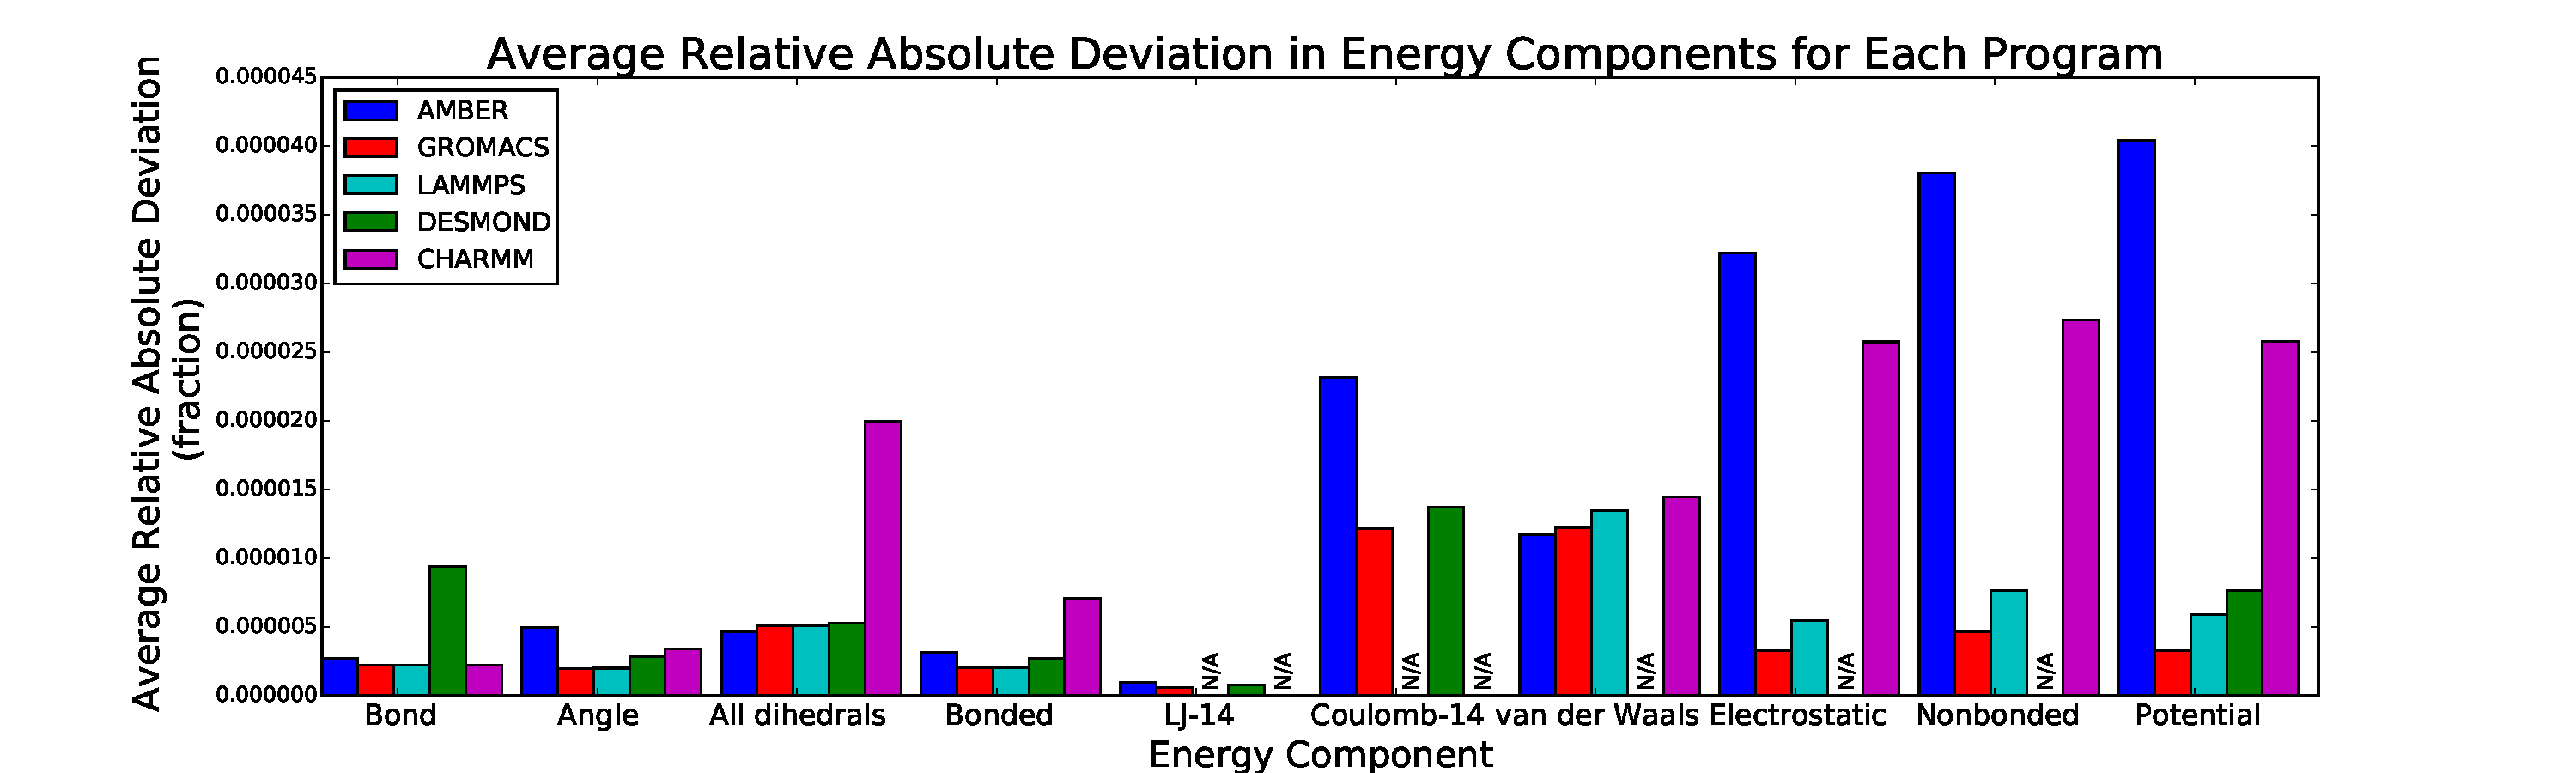
\includegraphics[width=\textwidth]{AverageRelativeAbsoluteIdealSettings.pdf}
\end{tabular}
\caption{We compare the variation of 10 different energy terms between
  five different simulation programs (AMBER, GROMACS, LAMMPS, DESMOND,
  and CHARMM) for the 'ideal' choice of cutoff parameters. For each
  term, we plot the deviation of each program from the average over
  all programs (the program average), to avoid choosing a single
  arbitrary reference program. All statistics are averaged over the 22
  SAMPL5 host-guest molecules. We plot the average deviation (top),
  the absolute average deviation (middle), and relative absolute
  average deviation (top).
\label{fig:mainfig}}
\end{figure}

We next examine the nonbonded interactions. Coulomb 1-4 and van der
Waals 1-4 interactions are a good measure of whether the nonbonded
parameters are being copied correctly, as they generally are all
calculated with real space interactions and are shorter range than any
reasonable cutoff. Therefore, their comparison is not affected by
nonbonded simulation parameter choices such as treatment of long-range
electrostatics and represents the best test of Lennard-Jones
interactions and charges are properly copied from one set of files to
another.

We see that, like the bonded interactions, the 1-4 interactions, when
separated out from other interactions by the simulation program, are
in good agreement.  In all available cases, the van der Waals 1-4
interactions have relative absolute differences at least a factor of 2
better than even the bond and angle interactions, at about 1 part in
10$^{-7}$. LAMMPS and CHARMM do not calculate 1-4 interactions
independently, but some post-processing tricks involving subtracting
energies with different input parameters show that the CHARMM van der
Waals 1-4 energies have similar accuracy, in particular being
generally within output precision of AMBER.

The story from the Coulombic 1-4 interactions is more
complicated. Looking at the absolute difference, we see that the
difference of GROMACS and DESMOND from the program average is about
half of what the difference is from AMBER. In this case, the
difference in Coulombic 1-4 interactions between GROMACS and DESMOND
is actually less than 10\% of what the differences is between AMBER
and the other two programs is, indicating that essentially all the
deviation from the program average is because of AMBER's difference
from the other two programs. Since the LJ 1-4 parameters are in good
agreement, the difference must come from some other source.

After some analysis of the data, it becomes clear that the value of
Coulomb's constant, the constant of proportionality $k$ in $U =
k\frac{q_1q_2}{r}$ is the cause of the differences in the Coulomb 1-4
terms. In Table~\ref{tab:delfromnist}, we show the value of the
Coulomb constant in a range of different simulation programs compared
to the NIST 2014 CODATA value.  We list ``AnteChamber'' instead of
{\tt sander} as in AMBER, the constant is set by multiplying the
charge by $\sqrt{k}$ in the {\tt .prmtop} file, rather than set
internally by the molecular dynamics engine.  Clearly, AnteChamber,
and to a lesser extent CHARMM, have significant deviation from the
best experimental value.  But how much does this deviation affect the
results?

\begin{table}
\caption{Values of Coulomb's law constant currently used in molecular
  simulation programs compared to the value of 332.06371302(32)
  calculated from NIST CODATA 2014. Specific versions of the programs
  used are described in the text. Two versions of GROMACS are listed
  because SAMPL5 energies were originally generated with version
  5.0.4, but the value has been changed since then. Coulomb's constant
  $f$ in units of kcal$\cdot$mol$^{-1}$ \AA e$^{-2}$ was calculated as
  $k_e N_A e^2$, where $k_e$ is Coulomb's constant defined exactly in
  N m$^2$C$^{-2}$, $N_a$ is Avogadro's number, and $e$ is the
  elementary charge from NIST CODATA 2014. [MRS: I'm using non-SI
    units because that's what actually hard coded in the programs, but
    can easily switch to be entirely in SI]. Uncertainties in $f$ were
  calculated using standard error propagation using NIST CODATA 2014
  values at the correlation coefficient between $N_A$ and $e$ of
  -0.9985, also from NIST CODATA 2014. At less than 1000 standard
  deviations, however, errors due to the Coulomb constant are no
  longer the largest source of error.\label{tab:delfromnist}}
% Coulomb's constant in kcal/mol A / elementary charge^2 / nm 
% f = k_e * N_a * e^2 * 10^10/4184 
% f/ke = N_a * e^2 \approx  e^2 dNa + 2 Na e de 
% (f/ke)^2 = e^4 dNa^2 + 4 Na^2 e^2 de^2 + 4 Na e^3 C dNa de
% where C is the correlation coefficient.  
\begin{tabular}{|ccc|}
\hline
Program & Value & $\sigma$ from NIST 2014 reference value \\
\hline
Antechamber &  332.0522173 & 51000 \\
GROMACS ($\leq$5.0) & 332.063693 & 89 \\
GROMACS ($>$5.1) & 332.0637138 & 3.3 \\ 
CHARMM & 332.054 & 43000 \\
LAMMPS & 332.06371 &  13 \\
DESMOND & 332.063762 & 220 \\
NAMD & 332.0636 & 510 \\
\hline
\end{tabular}
\end{table}

We test the effect of changes in the Coulomb law constant.  To add a
more rigorous control, we looking at the RMS difference in energy
between AMBER energies and GROMACS energies evaluated with it's 5.0.4
Coulomb constant, and then with GROMACS recompiled with the
AnteChamber Coulomb constant.  Results are shown in
Table~\ref{table:coulchange}. We see that matching Coulomb's constant
removes 98.8\% of the difference in the Coulomb 1-4 term between the
two programs, 69.5\% of the total electrostatic energy difference, and
74.2\% of the total potential energy difference between the two
programs, strongly indicating that the lack of agreement of AMBER with
the other programs is almost entirely a result of mismatched Coulomb's
law constants.

\begin{table}
\caption{RMSD in kJ/mol of different energy components in GROMACS
  5.0.4 from AMBER energies as GROMACS Coulomb constant is
  varied. Averages are calculated over all 22 SAMPL5 host-guest
  systems.~\label{table:coulchange}}
\begin{tabular}{|c|ccc|}
\hline
                          & Coulomb-14  & Electrostatic & Total Potential \\
\hline
GROMACS original constant &  0.00522    & 0.789         & 0.872  \\ 
AnteChamber constant      &  0.000064   & 0.241         & 0.225 \\
Percent difference explained & 98.8\%   & 69.5\%        & 74.2\% \\  
\hline
\end{tabular}
\end{table}

The longer range nonbonded interactions are significantly harder to
get in good agreement between programs.  Validating the van der Waals
and Coulombic 1-4 interactions demonstrates that the the Lennard-Jones
parameters and Coulombic charges are correctly created in the other
file formats.  In that sense, validating the conversion of file
formats can be done without comparing the long-range
interactions. However, if we are interested in comparing results of
molecular dynamics programs in realistic situations, we will need to
compare the entire potential energy, including these terms. [NOTE: at
  this point, we need to think about how important it is to answer
  this question, and whether this document can answer it sufficiently]

One complication is that different programs both calculate and print
out the different components of nonbonded interactions differently,
such as the direct space energy, the Fourier space energy, the Ewald
self term, and so forth.  Thus, it is often difficult to examine
anything except the total Lennard-Jones or total electrostatic
energy. This makes it hard to determine exactly the source of any
discrepancy between programs, and motivates our attempt to find
'ideal' simulation parameters to best make this comparison.

Discrepancies in the nonbonded energy terms are always much larger in
magnitude than discrepancies in the bonded interactions for any liquid
phase simulation, since there are many more intermolecular
interactions than intramolecular interactions.  It is therefore
instructive to look first at the average relative absolute deviations
from the program average. For GROMACS, AMBER, LAMMPS, and CHARMM, the
fractional difference in the van der Waals energy is approximately
$1\times 10^{-5}$, which is 2-5 times larger than the difference in
the bonded energy (DESMOND does not separate this energy out). GROMACS
and LAMMPS are generally closer to each other, usually within one part
in $10^6$, and CHARMM and AMBER are clustered together, though not as
closely as GROMACS and LAMMPS. Because of the close match of
Lennard-Jones 1-4 parameters, deviations are likely due to differences
in the calculation of long range interactions.

Differences from the program average in the total electrostatic energy
are smaller than errors in the total van der Waals energy for GROMACS
and LAMMPS, but are significantly larger for AMBER.  As seen above, a
large portion of the electrostatic deviation of AMBER from those two
programs is because of the inconsistent choice of Coulomb's constant.
Although CHARMM also has a relatively inaccurate Coulomb's constant,
the differences in the CHARMM potential energy are in the other
direction from AMBER, indicating a difference in the way the
electrostatic energy is calculated from the other programs.  [NOTE:
  this is the one place I'm a little worried about whether I am
  running a simulation correctly, and will follow up with CHARMM
  people] For AMBER, about 70\% of this deviation is due to the
Coulomb constant choice, leaving significantly less of the deviation
from other programs due to other choices in nonbonded simulation
parameters. An adjustment in CHARMM's Coulomb's constant would
actually make the energy further from the other three programs.
However, it is important to notice that this fraction difference is
still on the order of $2.5 \times 10^{-5}$, likely too small to matter
for most quantities of interest over long simulations.

The deviations in the program average of the total potential energy is
dominated by the differences in the nonbonded terms, since those are
so much larger than differences in the bonded energy.  For CHARMM and
AMBER, differences in the electrostatic nonbonded energy
dominates. DESMOND total potential energies differences from the
program average are almost the same as GROMACS and LAMMPS, indicating
that since the bonded interactions match the two programs well, the
nonbonded also must agree relatively well.

\begin{figure}[h]
\begin{tabular}{c}
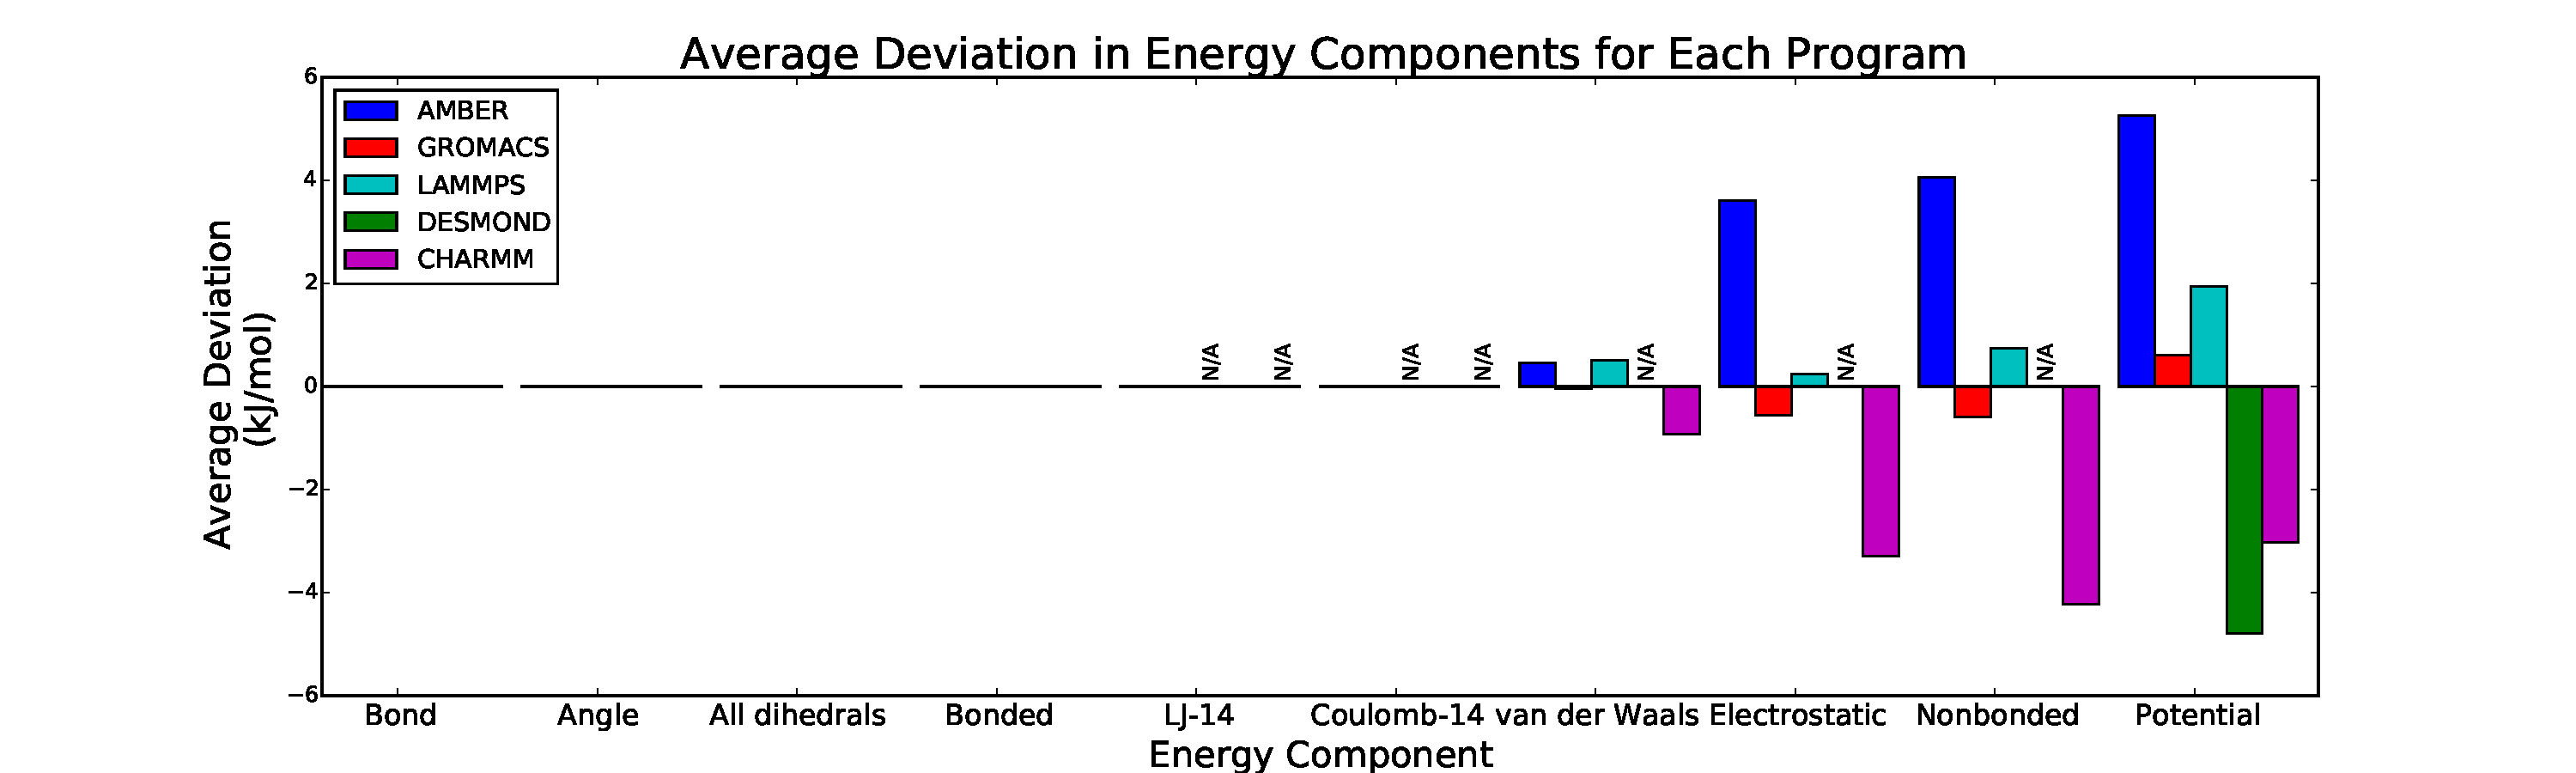
\includegraphics[width=\textwidth]{AverageDefaultSettings.pdf} \\  
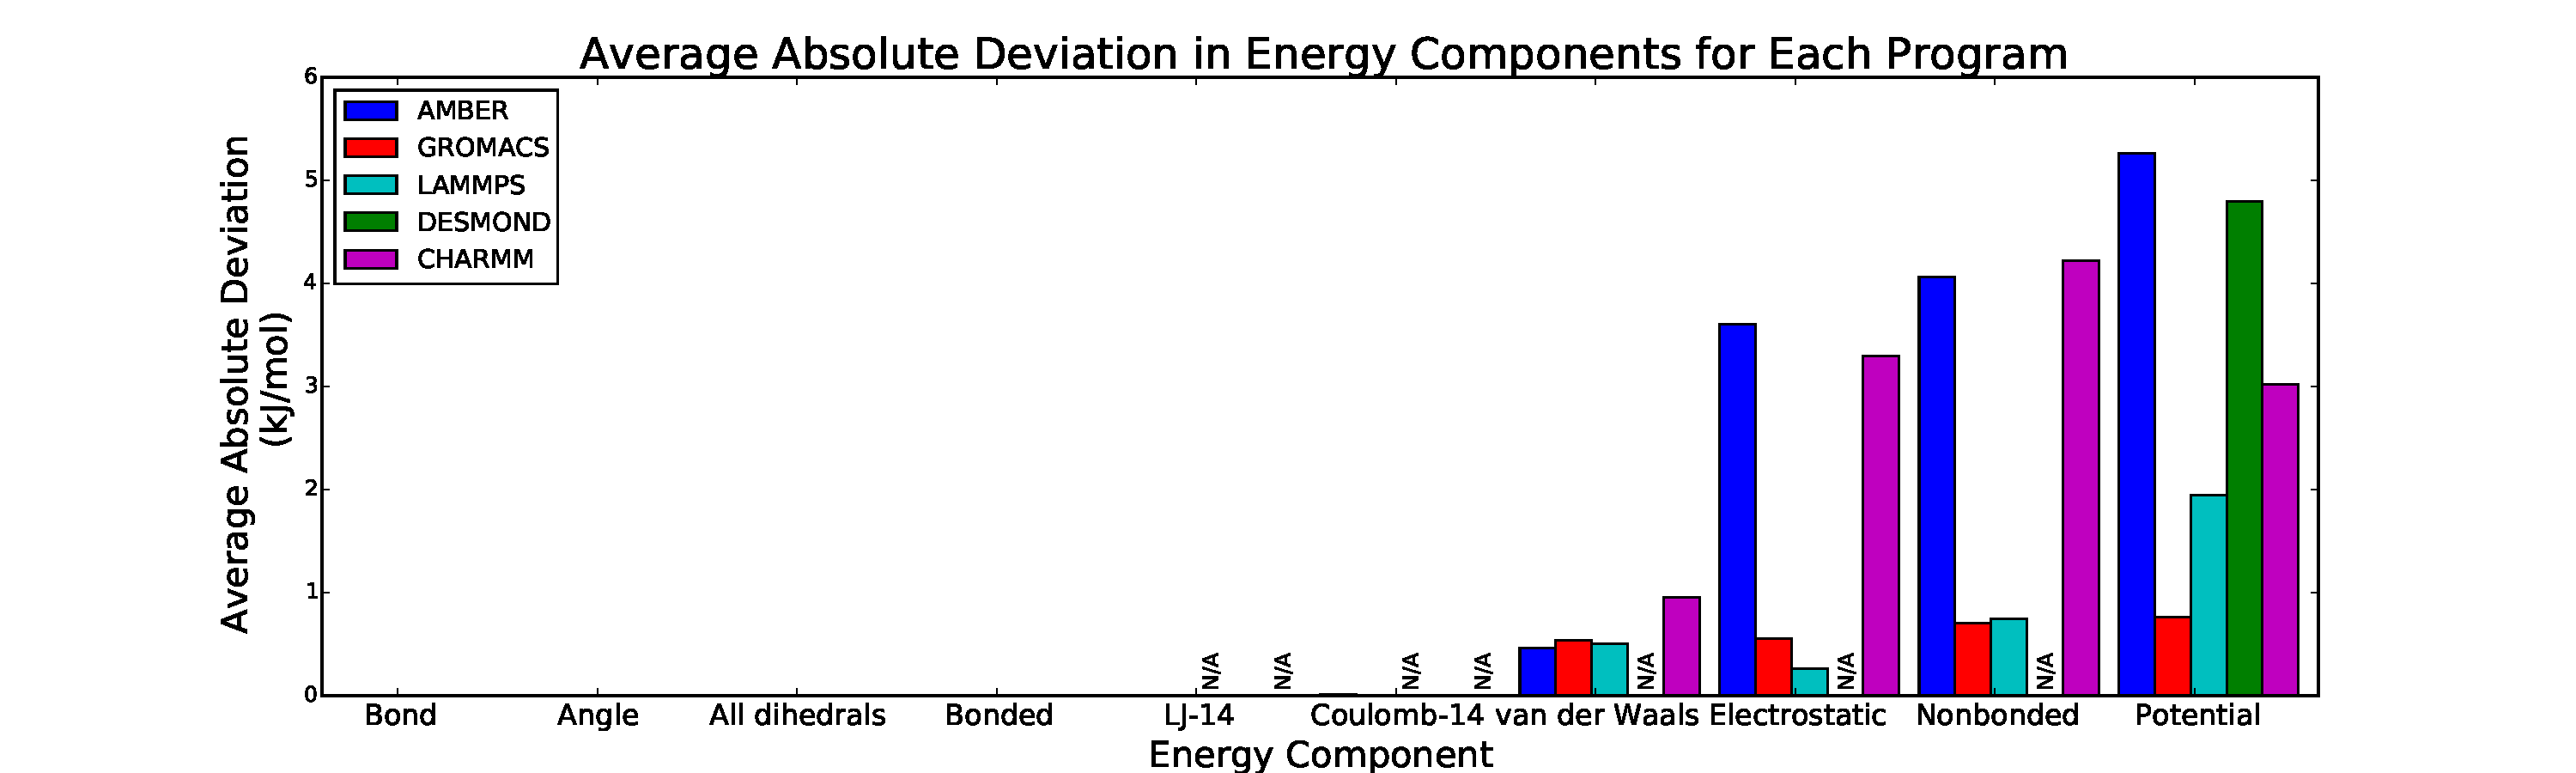
\includegraphics[width=\textwidth]{AverageAbsoluteDefaultSettings.pdf} \\  
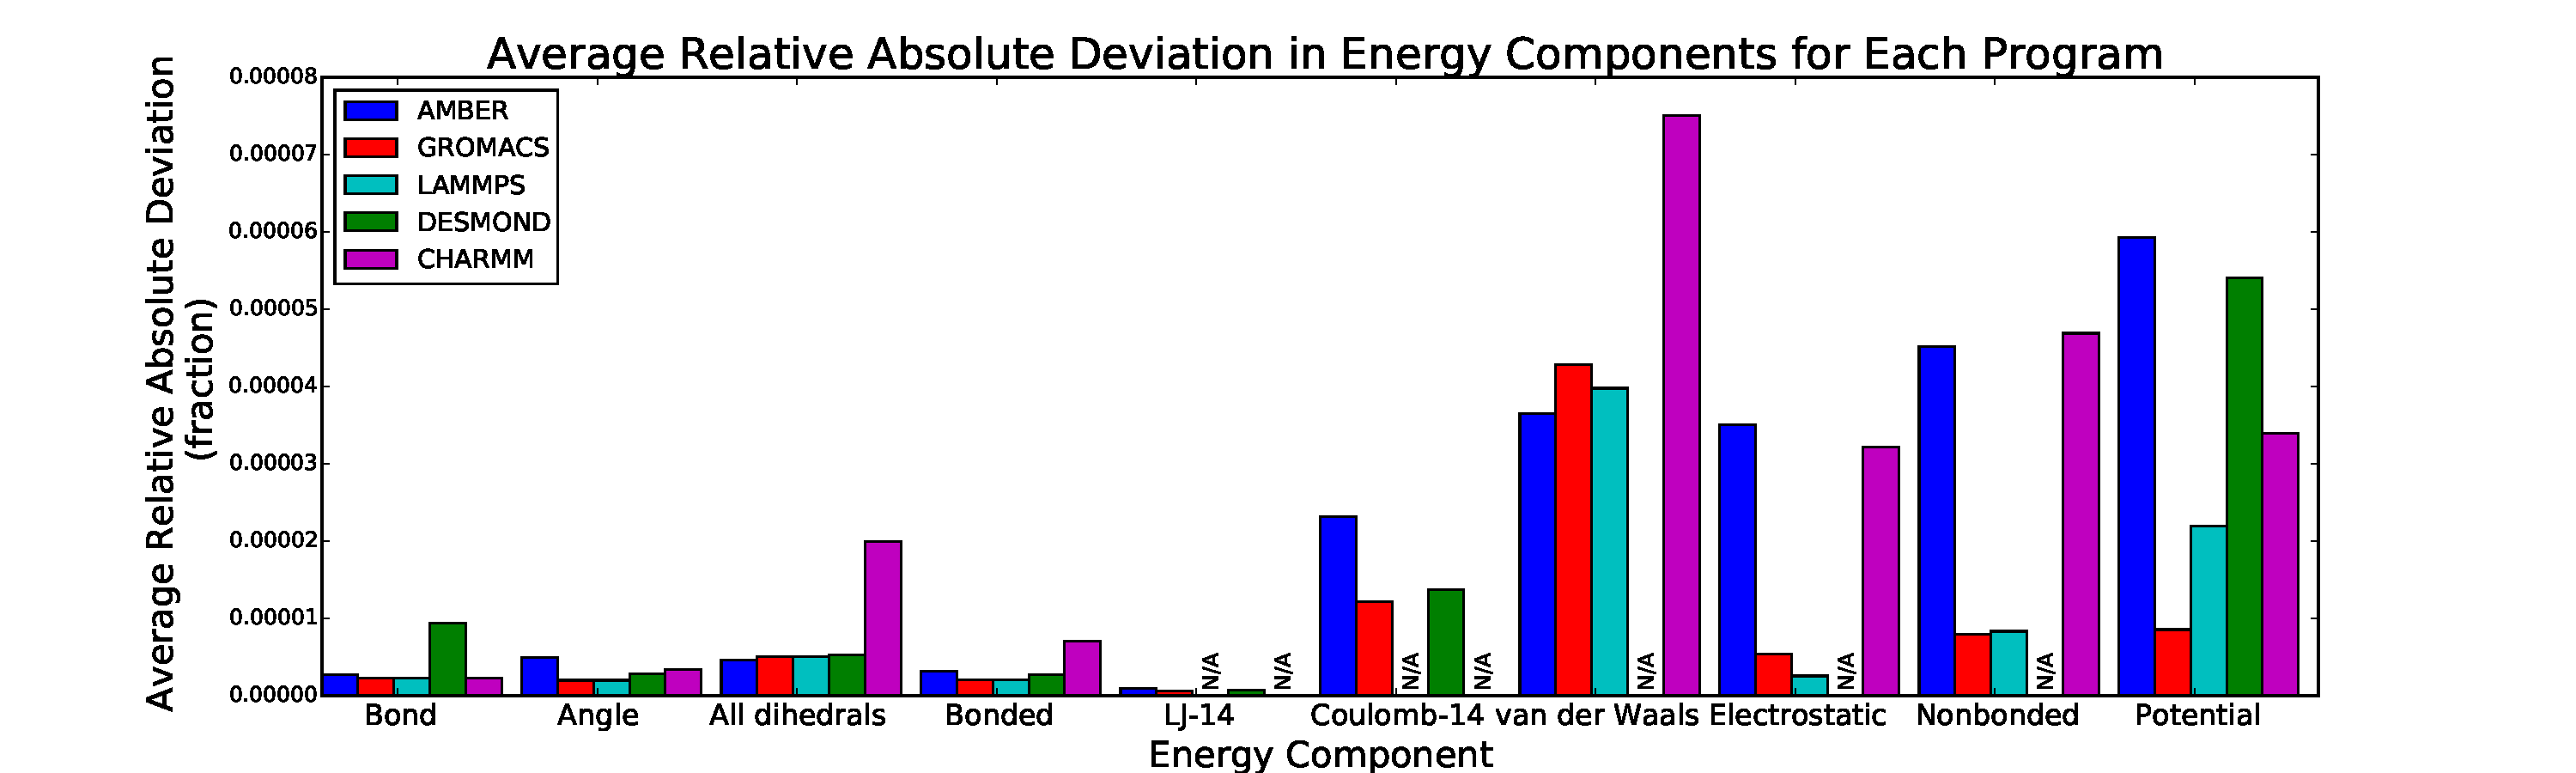
\includegraphics[width=\textwidth]{AverageRelativeAbsoluteDefaultSettings.pdf}
\end{tabular}
\caption{We compare the variation of 10 different energy terms between
  five different simulation programs (AMBER, GROMACS, LAMMPS, DESMOND,
  and CHARMM) for the 'default' choice of cutoff parameters (described
  in table). As above, for each term, we plot the deviation of each
  program from the average of all programs, to avoid choosing a single
  arbitrary reference program. All statistics are averaged over 22
  molecules. We plot the average deviation (top), the absolute average
  deviation (middle), and relative absolute average deviation
  (top). Nonbonded potential parameter deviations are approximately a
  factor of 2 larger than using the 'ideal' parameters.
\label{fig:defaultfig}}
\end{figure}

We also are interested in the deviations of energies as a function of
the number of coordinates used in the output file. The results of the
comparison between AMBER (full precision input) and GROMACS (reduced
precision output) are shown in Fig.~\ref{fig:precision}.  We choose
only to show GROMACS as the other programs show similar behavior. We
plot the $-\log_{10}$ of the average relative absolute difference
between the GROMACS energy and the AMBER energy as a function of the
number of decimal places in the output GROMACS coordinates from 8
digits after the decimal place (measured in nanometers) down to 4
after the decimal place, what one would obtain from a file downloaded
from the PDB.  We see that the total energy loses approximately 0.75-1
digits of relative precision in the energy for each digit of precision
of coordinate lost. Since the van der Waals and electrostatic
nonbonded energies contribute the majority of the potential energy,
their loss of precision mirrors the overall loss of
precision. Interestingly, the bonded and 1-4 terms are less sensitive
to changes in coordinate precision, not losing much precision until
getting down to 5 or fewer digits after the decimal point.  However,
losing just a few digits of precision completely washes out any other
source of error, demonstrating the importance of matching the
coordinates to high precision in order to validate the rest of the
conversion.

\begin{figure}[h]
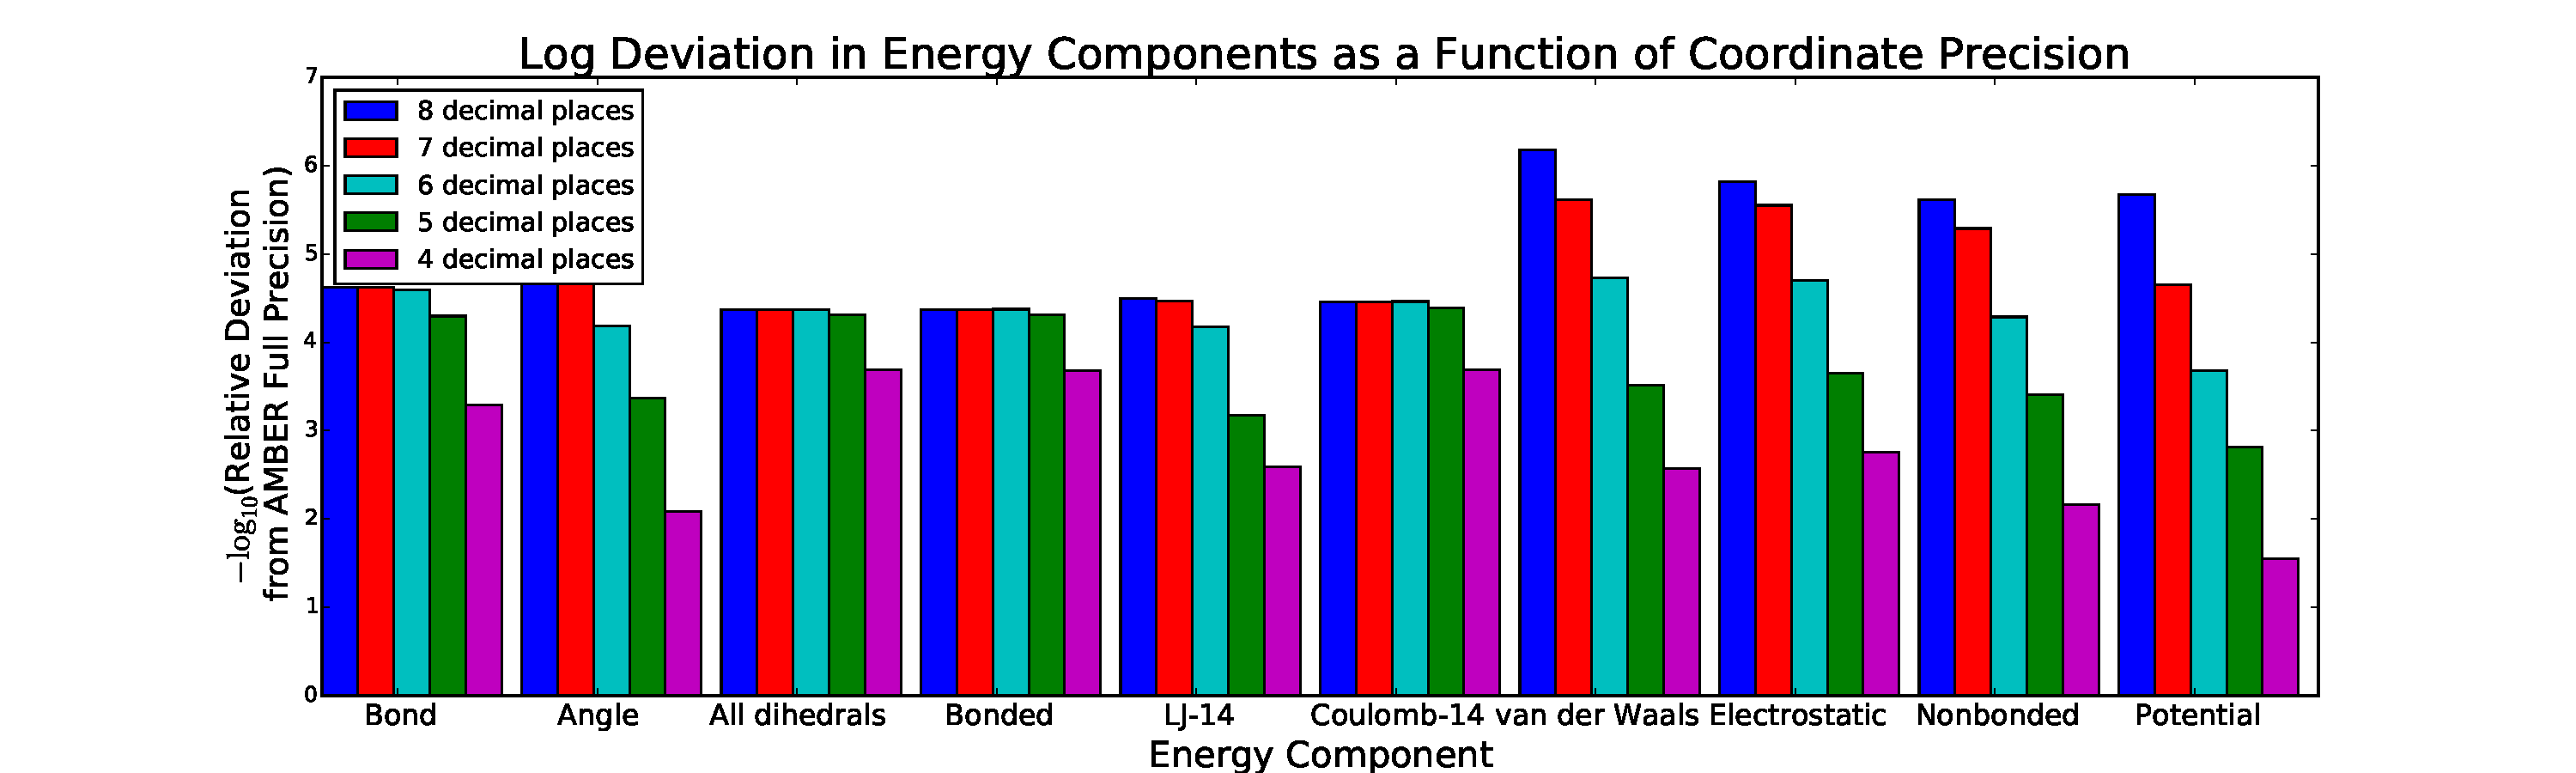
\includegraphics[width=\textwidth]{precisioncomparison.pdf}   
\caption{Matches in energy between converted files become rapidly
  worse as the number of digits of precision in the converted files
  decreases. We plot $-\log_{10}$ of the average relative absolute
  value in each energy term between AMBER and GROMACS, with fixed
  input coordinate precision, and variable output precision with the
  number of decimal places in the coordinates in nanometers, varying
  from 8 down to 4, the precision of a standard PDB file.
\label{fig:precision}}
\end{figure}

We are also interested in how much changing the precision of the
binaries affects energy comparisons.  We focus on the comparison
between single and double precision GROMACS, as it is specifically
designed to be compiled in either single and double precision, though
the single precision is the default version most simulations are run
with. In Table~\ref{fig:singlevdouble}, we compare the RMS differences
averaged over all 22 compounds between the two GROMACS binaries, AMBER
and single precision GROMACS, and AMBER and double precision GROMACS.
This comparison allows us to see both the magnitude of the difference
due to changes in binary precision, and how much this differences
affects the comparison to, for example, AMBER.

We see that the differences between single and double precision for
bonded terms is 2-8 times larger than the difference between AMBER and
double precision GROMACS, and is usually the dominant contribution to
the difference between AMBER and single precision GROMACS.
Differences between the precisions for LJ-14 is about equal to
differences between either precision and AMBER.  Differences between
precisions for Coulomb-14 terms is as low as the difference between
LJ-14, which is of course much less than the GROMACS to AMBER
difference, because of the previously described difference in Coulomb
constant. The differences in precision for the total van der Waals is
an order of magnitude lower than the difference between AMBER and
either GROMACS precision caused by differences in calculating the
long-range nonbonded terms.  However, single to double precision
change results in significant difference in the overall electrostatic
term, as large as the magnitude between GROMACS and AMBER.  Because
the total van der Waals energy changes relatively little between
precisions, it is likely that the short-range electrostatics (which
are functions only of the distance) are also relatively accurate, and
it is the Ewald summation part that changes upon changes in binary precision.

\begin{table}
\begin{tabular}{|c|ccc|}
\hline
E term & RMS($E_{single} - E_{double}$) &  RMS($E_{amber} - E_{single}$) &  RMS($E_{amber} - E_{double}$) \\
           Bond &   0.000066 &   0.000068 &   0.000008\\
          Angle &   0.000044 &   0.000043 &   0.000007\\
  All dihedrals &   0.000015 &   0.000031 &   0.000018\\
         Bonded &   0.000081 &   0.000086 &   0.000011\\
          LJ-14 &   0.000013 &   0.000020 &   0.000025\\
     Coulomb-14 &   0.000007 &   0.001250 &   0.001251\\
  van der Waals &   0.001894 &   0.021756 &   0.023116\\
  Electrostatic &   0.218874 &   0.403839 &   0.189265\\
      Nonbonded &   0.217209 &   0.422827 &   0.209207\\
      Potential &   0.217134 &   0.422781 &   0.209214\\
\hline
\end{tabular}
\caption{\label{fig:singlevdouble}Differences between double and
  single GROMACS energy evaluations are of similar magnitude to the
  differences between AMBER and GROMACS, but are dominated by
  differences in the long-range electrostatics. All energies in kJ/mol.}
\end{table}

We are also interested in how much of the differences between programs
vary with the configurations of each molecule. For example, if we were
to take different configurations of the same molecule, would we get
similar deviations from the program average for all of the molecules?
We ask this question by taking the 12 octa-acid hosts, and generating
20 configurations as described in the Methods section using NVT
molecular dynamics. The average over these 20 configurations is
therefore an rough approximation to the ensemble average energy of the
system.

We then compare the RMSD from the program average $\sigma_{config}$,
averaged over all $12 \times 20 = 240$ configurations, and the RMSD of
the average energy of all configurations of the same molecule from the
program average, averaged over the 12 host-guest
systems$~\sigma_{molecule}$. If the variation from program to program
is independent of configuration, and only dependent on the differences
between molecules, then we would expect that the two RMSDs would be
roughly equal (low conformation dependent variation).  If instead the
variation is independent of the specific molecule, then the RMSD from
the configurationally averaged deviations from program averages
($\sigma_{molecule}$ would be significantly smaller (approximately
$\sqrt{1/20} \approx 22$\% of the value). Note that the RMSD of the
conformationally averaged values must necessarily be lower than the
RMSD over all configurations and molecules. The extent to which it is
smaller shows how much of the variation is inherent to the molecules,
and how much is only dependent on the configurations.

We can quantify this difference in the source of variation by
calculating the fraction of the total variation due to conformational
variability, calculated as
$\frac{\sigma^2_{config}-\sigma^2_{molecule}}{\sigma^2_{molecule}}$,
for each energy term. If this quantity is low, then variation is
mostly due to differences between molecules, not configurations.  If
it is near one, then variation between programs is mostly due to
changes in conformation.

We can observe the results in Figure~\ref{fig:confvariability}. At one
extreme are the bond energies, which have only about 8\% of the total
variation between programs due to configurational variation, near the
minimum of 1/20 $\approx$ 5\%. Most of the differences are due to
differences between the molecular bond terms, but not the specific
conformation.  Similarly, the variations in van der Waals 1-4
interactions are mostly due to differences between molecules.

At the other extreme are the Coulomb 1-4 terms, where almost 100\% of
the variation is due to conformational variation: after averaging the
differences over molecules, there is very little variation left.
Similarly, almost 100\% of the variability in the total van der Waals
energy is due to conformational variability.  Variation in angle
energies from the program average again likely relatively dependent on
configuration (around 80\%). [NOTE: I don't entirely understand the
  differences between LJ-14 and Coulomb-14.  I need to think about it
  a bit more.]

Total electrostatic variation is one of the few energy components
where the fraction of conformational variation depends significantly
on the programs.  For AMBER, it is not very dependent on
configuration; for other programs, it is much more dependent on
configuration. This is likely because of differences in the Coulomb
constant and in the treatment of long-range electrostatic
energies. The long-range forces are much less dependent on individual
molecular distances, instead being dependent on the average
distribution of charge within the system, which does not change
significantly for a host-guest system over time, and which will scale
with the changes in the Coulomb constant.  On the other hand, the
Coulomb 1-4 interactions are dominated by the variability of which
atoms are closest to each other at any given time.

The analysis in the variation of the total potential energy conclusion
illustrates again that the dominant reason that the molecular
simulations differ are the evaluation of long-range interactions,
especially the electrostatics, and the choice of the Coulomb
constant. We find that the total variation of the potential energy,
like total potential energy itself, depends almost entirely on the
nonbonded terms.  Since the van der Waals variation between programs
is almost entirely conformation dependent, with very little deviation
in programs between the ensemble average estimate for each molecule,
the conformational dependence of the total energy is essentially
determined by the conformational dependence of the electrostatic
energy. The bonded terms are essentially irrelevant.


\begin{figure}[h]
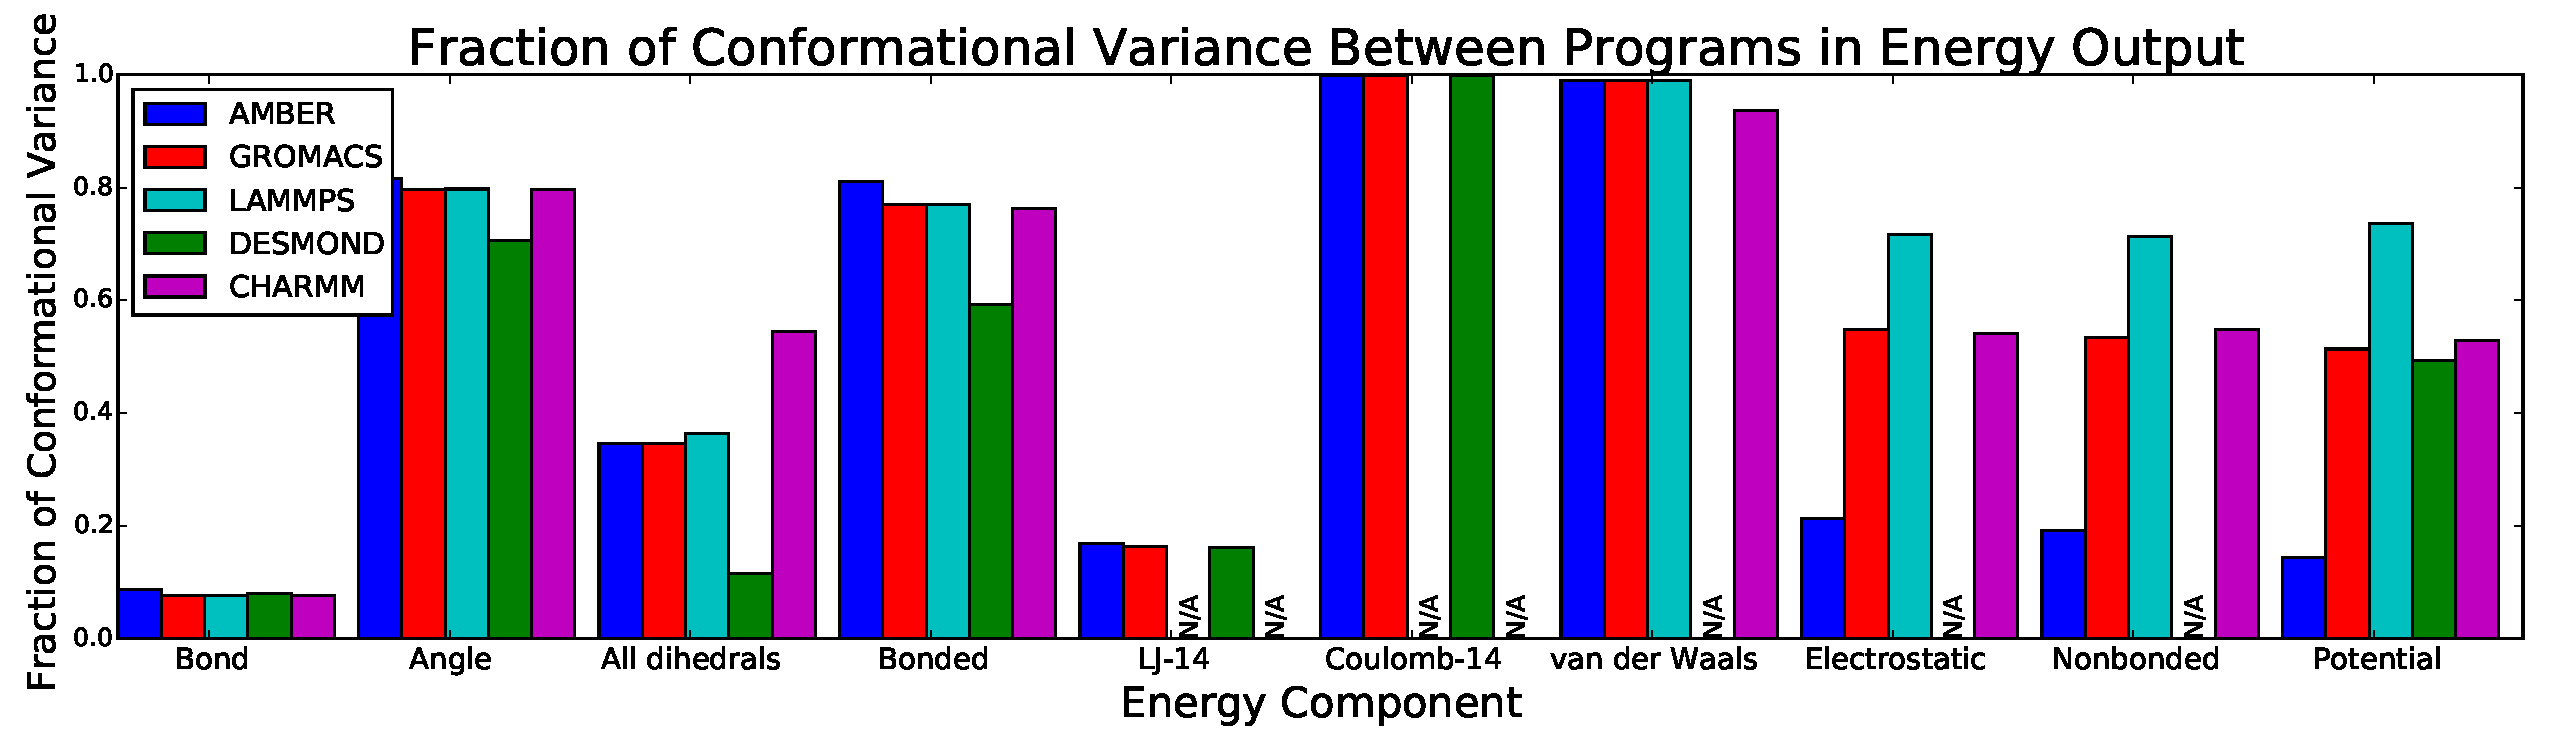
\includegraphics[width=\textwidth]{fractionofvariation.pdf}   
\caption{Fraction of variation from the program average due to
  conformational variability instead of molecular variability.
\label{fig:confvariability}}
\end{figure}

\section*{Discussion}

\subsection*{Issues in file conversion}
Creating true all-to-all functionality is particularly
difficult. There are a number of one-to-one conversion utilities and
scripts: for example, ACPYPE~\cite{sousa_da_silva_acpype_2012},
CHAMBER~\citep{crowley_chamber:_2009}, and {\tt amber2lmp}.  We have
developed InterMol and ParmEd as all-to-all converters, though neither
yet manages to interact with all programs.

Some important tools have enabled more general conversion. Both
InterMol and ParmEd automatically convert units between simulation
input files, removing the needs for manual unit conversion. This is
handled by creating data classes that carry units with them, making
conversion much simpler.  We believe that this study represents the
largest automated comparison between different programs that has been
performed so far, a process only possible because of the automated
conversion.

There are a number of differences between programs not immediately
obvious that nonetheless need to be carefully matched.  For example,
GROMACS builds lists of 1-4 interaction based on the bond topology: if
three bonds connect two atoms, they are 1-4 interactions. However,
AMBER uses the presence of dihedrals to define 1-4 interactions. A
dihedral with zero energy in GROMACS is essentially redundant and can
be eliminated without affecting the energy, but creates 1-4
interactions in AMBER.

\subsection*{Issues in matching energies}

It is difficult to say what the ``right'' energy is for a system, as
there are several different reasonable choices for implementation of
long-range interactions. For a sufficiently large box, one could
simply extend out the cutoffs, treating an increasingly larger amount
of the system using straight forward short-range interactions.
However, these systems, at 4.0 nm across, are not large enough to
completely converge.

[NOTE: I could build a really big box of water and see which
  simulation approach converged best to really long short range
  cutoffs, and rank the approaches that way.]

It is difficult to assign a label ``proper'' or ``improper'' to a
given dihedral, since in different programs the same functional form
is used for both types. We thus put all of the energy together as
dihedral energy when reporting them to avoid having to deal with the
ambiguity of different decompositions.

The results presented here strongly suggest that all molecular
simulation programs should choose a sufficiently consistent value for
Coulomb's constant. A value off of experiment by 0.01 is simply not
accurate enough to allow simulations to agree.  The results presented
here suggest that once the deviation is below 0.0001, any additional
error contributes less than other sources of error, so a value of
332.06371$\pm$0.00005 should reduce this sort of discrepancy below the
level of differences created by other programs.  This level of
agreement is present in all current programs with the exception of
CHARMM and AMBER, with GROMACS, at the edge of that range, recently
improving the precision by a factor of 4 in the 5.1 release.

Other than the difference in Coulomb's law, most programs agree quite
well, likely enough for most practical purposes as most thermodynamic
quantities cannot be measured that accurately.  All conversions were
performed accurately and the model parameter conversion was validated
to high precision. Only the long-range interactions deviated by
moderate amounts between programs, especially the electrostatic
Fourier-space interactions.  Even those differences are unlikely to
affect most thermodynamics studies.


\begin{acknowledgements}
The authors would like to thank Frank Pickard (NIH) for sample CHARMM
inputs and discussion about evaluation of CHARMM energies, Justin
Lemkul (U. Maryland) for advice on CHARMM functional form, and Michael
Zhu (U. Va.), Hari Devanathan (U. Va.), and Jacob Rosenthal (U. Va.)
for initial work on InterMol.
\end{acknowledgements}

% BibTeX users please use one of
\bibliographystyle{spjcamd}
%\bibliographystyle{spbasic}      % basic style, author-year citations
%\bibliographystyle{spmpsci}      % mathematics and physical sciences
%\bibliographystyle{spphys}       % APS-like style for physics
\bibliography{JCAMD_citations,Zotero}   % name your BibTeX data base

% Non-BibTeX users please use
%\begin{thebibliography}{}
%
% and use \bibitem to create references. Consult the Instructions
% for authors for reference list style.
%
%\bibitem{RefJ}
% Format for Journal Reference
%Author, Article title, Journal, Volume, page numbers (year)
% Format for books
%\bibitem{RefB}
%Author, Book title, page numbers. Publisher, place (year)
% etc
%\end{thebibliography}

\end{document}
% end of file template.tex


% LocalWords:  tex SVJour EPS cucurbit uril octa der waals vdW SAMPL PACS MSC
% LocalWords:  nominalizations CB OA Moghaddam Muddana Gallicchio Jayachandran
% LocalWords:  Lyubartsev Escobedo Desgranges solute Christoph Swails Jian TN
% LocalWords:  Gilson Zhong Skaggs San CA VA GROMACS LAMMPS CHARMM ParmEd NVE
% LocalWords:  InterMol Coulomb's deconvolute microcanonical NVT limitating NJ
% LocalWords:  Lennard SPME kJ acepype intercoversion py API nonbonded CBClip
% LocalWords:  OAH OAMe MOE sulfonic carboxylic protonation pKas RESP HF Joung
% LocalWords:  Antechamber atm solutes SI odinger dms cms charmm lite RHEL gcc
% LocalWords:  PPPM CC lj Langevin timestep nonbondeds html nx ny nz doesn Rtol
% LocalWords:  tol coul pre lammps CCCCCCCCCC NIST CODATA Avogadro's ke dNa Na
% LocalWords:  de NAMD Pickard NIH Justin Lemkul Zhu Hari Devanathan Va BibTeX
% LocalWords:  APS JCAMD RefJ RefB rst Schr al geballe sampl guthrie hess wu da
% LocalWords:  gromacs plimpton essmann sousa silva crowley lmp gui acpype
% LocalWords:  wang AllenAndTildesley dihedrals CHARMM's RMSDs Adittionally
% LocalWords:  parameteters AnteChamber intramolecular nanometers AMBER's
% LocalWords:  configurationally Zotero prmtop n
